\chapter{Stereo Vision}
\label{stereo}

% **************************** Define Graphics Path **************************
\graphicspath{{Chapter4/Figs/}}


%%%%%%%%% BODY TEXT
\section{Introduction}

{\let\thefootnote\relax\footnote{{In this Chapter, \cref{stereo_literature}, \cref{section:model} and \cref{section:evaluation} was collaborative work with Hayk Martirosyan, Saumitro Dasgupta, Peter Henry, Ryan Kennedy, Abraham Bachrach, and Adam Bry and was published in \citep{kendall2017end}}}}

\begin{figure*}[t]
	\begin{center}
		\includegraphics[width=\linewidth]{deep_stereo}
	\end{center}
	\caption[An end-to-end deep learning model for stereo regression.]{\textbf{Our end-to-end deep stereo regression architecture, GC-Net} (\underline{G}eometry and \underline{C}ontext \underline{Net}work).}
	\label{fig:model}
\end{figure*}

Accurately estimating three dimensional geometry from stereo imagery is a core problem for many computer vision applications, including autonomous vehicles and UAVs \citep{achtelik2009stereo}. Stereo algorithms typically estimate the difference in the horizontal position of an object between a rectified pair of stereo images. This is known as \textit{disparity}, which is inversely proportional to the scene depth at the corresponding pixel location. In this chapter we are specifically interested in computing the disparity of each pixel between a rectified stereo pair of images. 

To achieve this, the core task of a stereo algorithm is computing the correspondence of each pixel between two images. This is very challenging to achieve robustly in real-world scenarios. Current state-of-the-art stereo algorithms often have difficulty with textureless areas, reflective surfaces, thin structures and repetitive patterns. Many stereo algorithms aim to mitigate these failures with pooling or gradient based regularization \citep{geiger2010efficient,hirschmuller2005accurate}. However, this often requires a compromise between smoothing surfaces and detecting detailed structures.

In contrast, deep learning models have been successful in learning powerful representations directly from the raw data in object classification \citep{krizhevsky2012imagenet}, detection \citep{girshick2014rich} and semantic segmentation \citep{long2015fully,badrinarayanan2017segnet}. These examples demonstrate that deep convolutional networks are very effective for understanding semantics. They excel at classification tasks when supervised with large training datasets. We observe that a number of these challenging problems for stereo algorithms would benefit from knowledge of global semantic context, rather than relying solely on local geometry. For example, given a reflective surface of a vehicle's wind-shield, a stereo algorithm is likely to be erroneous if it relies solely on the local appearance of the reflective surface to compute geometry. Rather, it would be advantageous to understand the semantic context of this surface (that it belongs to a vehicle) to infer the local geometry. In this chapter we show how to learn a stereo regression model end-to-end, with the capacity to understand wider contextual information.

Stereo algorithms which leverage deep learning representations have so far been largely focused on using them to generate unary terms \citep{zbontar2015computing,luo2016efficient}. Applying cost matching on the deep unary representations performs poorly when estimating pixel disparities \citep{luo2016efficient,zbontar2015computing}. Traditional regularization and post processing steps are still used, such as semi global block matching and left-right consistency checks \citep{hirschmuller2005accurate}. These regularization steps are severely limited because they are hand-engineered, shallow functions, which are still susceptible to the aforementioned problems.

This chapter asks the question, can we formulate the entire stereo vision problem with deep learning using our understanding of stereo geometry? The main contribution of this chapter is an end-to-end deep learning method to estimate per-pixel disparity from a single rectified image pair. Our architecture is illustrated in \fig{model}. It explicitly reasons about geometry by forming a cost volume, while also reasoning about semantics using a deep convolutional network formulation. We achieve this with two key ideas:
\begin{itemize}
\item We learn to incorporate context directly from the data, employing 3-D convolutions to learn to filter the cost volume over $height\times width\times disparity$ dimensions,
\item We use a soft argmin function, which is fully differentiable, and allows us to regress sub-pixel disparity values from the disparity cost volume.
\end{itemize}

\cref{section:model} introduces this model. In \cref{section:evaluation} we evaluate our model on the synthetic Scene Flow dataset \citep{MIFDB16} and set a new state-of-the-art benchmark on the KITTI 2012 and 2015 datasets \citep{Geiger2012CVPR,Menze2015CVPR}. Finally, in \cref{sec:saliency} we present evidence that our model has the capacity to learn semantic reasoning and contextual information.


In the remainder of this chapter, we demonstrate how to jointly learn depth from labelled and unlabelled data. We get the best of both worlds, leveraging labels to learn accurate disparities and large cohorts of unlabelled data for robustness. We do this by approaching the problem with a thorough probabilistic treatment. We make the observation that unsupervised learning can provide a strong signal for learning in many regions that supervised models find difficult -- such as occlusion boundaries and thin structures, where there is a strong photometric discontinuity. However, regions which suffer from the aperture problem, such as sky and other flat, texture-less regions, are easier to solve with supervised learning. We show how to use recent advances in probabilistic deep learning to leverage the most informative signal from each training mode, and attenuate more uncertain areas.

To achieve this, we model uncertainty in stereo vision using \textit{probabilistic deep learning}, which provides a framework for understanding uncertainty with deep learning models \citep{kendall2017uncertainties,gal2016thesis} and was introduced in \cref{scene_understanding}. In \sct{unc_model} we show how to form an architecture which learns to regress stereo disparities and \textit{heteroscedastic} (data dependent) uncertainty \citep{der2009aleatory} from a rectified stereo pair of images. Our method does not require labels for uncertainty, rather it is learned implicitly from the data.

In summary, the main contributions of this chapter are:
\begin{enumerate}
\item forming an end-to-end model for stereo disparity regression which explicitly uses geometry,
\item advancing state-of-the-art on the Kitti stereo benchmark \citep{Geiger2012CVPR},
\item demonstrating how to model uncertainty in stereo vision with probabilistic deep learning,
\item showing how to combine labelled and unlabelled data with semi-supervised learning.
\end{enumerate}

\section{Literature Review}
\label{stereo_literature}

The problem of computing depth from stereo image pairs has been studied for quite some time~\citep{Barnard1982}. Stereo algorithms typically estimate the difference in the horizontal position of an object between a rectified pair of stereo images. This is known as \textit{disparity}, which is inversely proportional to the scene depth at the corresponding pixel location. A survey by Scharstein and Szeliski~\citep{scharstein2002taxonomy} provides a taxonomy of stereo algorithms as performing some subset of: matching cost computation, cost support aggregation, disparity computation and optimization, or disparity refinement. This survey also described the first Middlebury dataset and associated evaluation metrics, using structured light to provide ground truth.  
An improved higher resolution Middlebury dataset was presented in~\citep{Scharstein2014}. 
The KITTI dataset~\citep{Geiger2012CVPR,Menze2015CVPR} is a larger dataset from data collected from a moving vehicle with LIDAR ground truth. These datasets first motivated improved hand-engineered techniques for all components of stereo, of which we mention a few notable examples.

The matching cost is a measure of pixel dissimilarity for potentially corresponding objects across stereo images \citep{Hirschmuller2007}. The matching cost does not provide a measure of uncertainty, rather it predicts the relative likelihood between various disparity solutions. Traditionally, local descriptors based on gradients~\citep{geiger2010efficient} or binary patterns, such as CENSUS~\citep{Zabih1994} or BRIEF~\citep{Calonder2010,Heise2015}, have been used. More recently, machine learning techniques have been applied to estimate stereo correspondences; Markov random fields \citep{Zhang2007}, conditional random fields \citep{Scharstein2007}, support vector machines \citep{Li2008} and deep learning \citep{zbontar2015computing,Zagoruyko2015} have all been shown to be increasingly effective. Recent deep learning advances have improved performance by matching image patches using a Siamese network \citep{luo2016efficient}, multi-scale embeddings \citep{chen2015deep}.

Local matching costs often require post processing or regularization, which attempts to incorporate knowledge of the global context \citep{Kolmogorov2001,Klaus2006,Bleyer2011}. A common technique is \emph{Semi-Global Matching} (SGM) \citep{Hirschmuller2008} which uses dynamic programming to optimize the path-wise form of the energy function in many directions.

In addition to providing a basis for comparing stereo algorithms, the ground truth depth data from these datasets provides the opportunity to use machine learning for improving stereo algorithms in a variety of ways.  Zhang and Seitz~\citep{Zhang2007} alternately optimized disparity and Markov random field regularization parameters.  Scharstein and Pal~\citep{Scharstein2007} learn conditional random field (CRF) parameters, and Li and Huttenlocher~\citep{Li2008} train a non-parametric CRF model using the structured support vector machine.  Learning can also be employed to estimate the confidence of a traditional stereo algorithm, such as the random forest approach of Haeusler et al.~\citep{Haeusler2013a}.  Such confidence measures can improve the result of SGM as shown by Park and Yoon~\citep{Park2015}.

Deep convolutional neural networks can be trained to match image patches~\citep{Zagoruyko2015}.  A deep network trained to match $9 \times 9$ image patches, followed by non-learned cost aggregation and regularization, was shown by {\v Z}bontar and LeCun~\citep{zbontar2015computing,zbontar2016stereo} to produce then state-of-the-art results.  Luo et al. presented a notably faster network for computing local matching costs as a multi-label classification of disparities using a Siamese network~\citep{luo2016efficient}.  A multi-scale embedding model from Chen et al.~\citep{chen2015deep} also provided good local matching scores.  Also noteworthy is the \emph{DeepStereo} work of Flynn et al.~\citep{Flynn2016}, which learns a cost volume combined with a separate conditional colour model to predict novel viewpoints in a multi-view stereo setting.

Mayer et al. created a large synthetic dataset to train a network for disparity estimation (as well as optical flow)~\citep{MIFDB16}, improving the state-of-the-art. As one variant of the network, a 1-D correlation was proposed along the disparity line which is a multiplicative approximation to the stereo cost volume. In contrast, our work does not collapse the feature dimension when computing the cost volume and uses 3-D convolutions to incorporate context.

Though the focus of this work is on binocular stereo, it is worth noting that the representational power of deep convolutional networks also enables depth estimation from a single monocular image~\citep{eigen2014depth}.  Deep learning is combined with a continuous CRF by Liu et al.~\citep{Liu2015}.  Instead of supervising training with labelled ground truth, unlabelled stereo pairs can be used to train a monocular model~\citep{garg2016unsupervised}.

In our work, we apply no post-processing or regularization. We explicitly reason about geometry by forming a fully differentiable cost volume and incorporate context from the data with a 3-D convolutional architecture.  We don't learn a probability distribution, cost function, or classification result.  Rather, our network is able to directly regress a sub-pixel estimate of disparity from a stereo image pair.

\section{Learning End-to-End Disparity Regression}
\label{section:model}

Rather than design any step of the stereo algorithm by hand, we would like to learn an end-to-end mapping from an image pair to disparity maps using deep learning. We hope to learn a more optimal function directly from the data. Additionally, this approach promises to reduce much of the engineering design complexity. However, our intention is not to naively construct a machine learning architecture as a black box to model stereo. Instead, we advocate the use of the insights from many decades of multi-view geometry research \citep{hartley2000} to guide architectural design. Therefore, we form our model by developing differentiable layers representing each major component in traditional stereo pipelines \citep{scharstein2002taxonomy}. This allows us to learn the entire model end-to-end while leveraging our geometric knowledge of the stereo problem. 

Our architecture, GC-Net (\underline{G}eometry and \underline{C}ontext \underline{Net}work) is illustrated in \fig{model}, with a more detailed layer-by-layer definition in \tbl{model}. In the remainder of this section we discuss each component in detail. Later, in Section \ref{sec:model_results}, we present quantitative results justifying our design decisions.

\begin{table}[p]
\centering
\clearpage
\begin{tabular}{l|l|c}
& Layer Description & Output Tensor Dim. \\ \hline \hline
& Input image & H$\times$W$\times$C \\ \hline
\multicolumn{3}{c}{\textbf{Unary features (section \ref{sec:unary})}} \\ \hline
1 & 5$\times$5 conv, 32 features, stride 2 & \sfrac{1}{2}H$\times$\sfrac{1}{2}W$\times$F \\
2 & 3$\times$3 conv, 32 features & \sfrac{1}{2}H$\times$\sfrac{1}{2}W$\times$F \\
3 & 3$\times$3 conv, 32 features & \sfrac{1}{2}H$\times$\sfrac{1}{2}W$\times$F \\
 & add layer 1 and 3 features (residual connection) & \sfrac{1}{2}H$\times$\sfrac{1}{2}W$\times$F \\
4-17 & (repeat layers 2,3 and residual connection) $\times$ 7 & \sfrac{1}{2}H$\times$\sfrac{1}{2}W$\times$F \\
%  & dropout & \sfrac{1}{2}H$\times$\sfrac{1}{2}W$\times$F \\
18 & 3$\times$3 conv, 32 features, (no ReLu or BN) & \sfrac{1}{2}H$\times$\sfrac{1}{2}W$\times$F \\ \hline
\multicolumn{3}{c}{\textbf{Cost volume (section \ref{sec:cost_vol})}} \\ \hline
 & Cost Volume & \sfrac{1}{2}D$\times$\sfrac{1}{2}H$\times$\sfrac{1}{2}W$\times$2F \\ \hline
\multicolumn{3}{c}{\textbf{Learning regularization (section \ref{sec:regularise})}} \\ \hline
%
19 & 3-D conv, 3$\times$3$\times$3, 32 features & \sfrac{1}{2}D$\times$\sfrac{1}{2}H$\times$\sfrac{1}{2}W$\times$F \\
20 & 3-D conv, 3$\times$3$\times$3, 32 features & \sfrac{1}{2}D$\times$\sfrac{1}{2}H$\times$\sfrac{1}{2}W$\times$F \\
%  & dropout & \sfrac{1}{2}D$\times$\sfrac{1}{2}H$\times$\sfrac{1}{2}W$\times$F \\
%
21 & From Cost Volume: 3-D conv, 3$\times$3$\times$3, 64 features, stride 2 & \sfrac{1}{4}D$\times$\sfrac{1}{4}H$\times$\sfrac{1}{4}W$\times$2F \\
%
22 & 3-D conv, 3$\times$3$\times$3, 64 features & \sfrac{1}{4}D$\times$\sfrac{1}{4}H$\times$\sfrac{1}{4}W$\times$2F \\
23 & 3-D conv, 3$\times$3$\times$3, 64 features & \sfrac{1}{4}D$\times$\sfrac{1}{4}H$\times$\sfrac{1}{4}W$\times$2F \\
%  & dropout & \sfrac{1}{4}D$\times$\sfrac{1}{4}H$\times$\sfrac{1}{4}W$\times$F \\
%
24 & From 21: 3-D conv, 3$\times$3$\times$3, 64 features, stride 2 & \sfrac{1}{8}D$\times$\sfrac{1}{8}H$\times$\sfrac{1}{8}W$\times$2F \\
%
25 & 3-D conv, 3$\times$3$\times$3, 64 features & \sfrac{1}{8}D$\times$\sfrac{1}{8}H$\times$\sfrac{1}{8}W$\times$2F \\
26 & 3-D conv, 3$\times$3$\times$3, 64 features & \sfrac{1}{8}D$\times$\sfrac{1}{8}H$\times$\sfrac{1}{8}W$\times$2F \\
%  & dropout & \sfrac{1}{8}D$\times$\sfrac{1}{8}H$\times$\sfrac{1}{8}W$\times$F \\
%
27 & From 24: 3-D conv, 3$\times$3$\times$3, 64 features, stride 2 & \sfrac{1}{16}D$\times$\sfrac{1}{16}H$\times$\sfrac{1}{16}W$\times$2F\\
%
28 & 3-D conv, 3$\times$3$\times$3, 64 features & \sfrac{1}{16}D$\times$\sfrac{1}{16}H$\times$\sfrac{1}{16}W$\times$2F \\
29 & 3-D conv, 3$\times$3$\times$3, 64 features & \sfrac{1}{16}D$\times$\sfrac{1}{16}H$\times$\sfrac{1}{16}W$\times$2F \\
%  & dropout & \sfrac{1}{16}D$\times$\sfrac{1}{16}H$\times$\sfrac{1}{16}W$\times$F \\
%
30 & From 27: 3-D conv, 3$\times$3$\times$3, 128 features, stride 2 & \sfrac{1}{32}D$\times$\sfrac{1}{32}H$\times$\sfrac{1}{32}W$\times$4F\\
%
31 & 3-D conv, 3$\times$3$\times$3, 128 features & \sfrac{1}{32}D$\times$\sfrac{1}{32}H$\times$\sfrac{1}{32}W$\times$4F \\
32 & 3-D conv, 3$\times$3$\times$3, 128 features & \sfrac{1}{32}D$\times$\sfrac{1}{32}H$\times$\sfrac{1}{32}W$\times$4F \\
%  & dropout & \sfrac{1}{32}D$\times$\sfrac{1}{32}H$\times$\sfrac{1}{32}W$\times$F \\
%
33 & 3$\times$3$\times$3, 3-D transposed conv, 64 features, stride 2 & \sfrac{1}{16}D$\times$\sfrac{1}{16}H$\times$\sfrac{1}{16}W$\times$2F \\
 & add layer 33 and 29 features (residual connection) & \sfrac{1}{16}D$\times$\sfrac{1}{16}H$\times$\sfrac{1}{16}W$\times$2F \\
%
34 & 3$\times$3$\times$3, 3-D transposed conv, 64 features, stride 2 & \sfrac{1}{8}D$\times$\sfrac{1}{8}H$\times$\sfrac{1}{8}W$\times$2F \\
 & add layer 34 and 26 features (residual connection) & \sfrac{1}{8}D$\times$\sfrac{1}{8}H$\times$\sfrac{1}{8}W$\times$2F \\
%
35 & 3$\times$3$\times$3, 3-D transposed conv, 64 features, stride 2 & \sfrac{1}{4}D$\times$\sfrac{1}{4}H$\times$\sfrac{1}{4}W$\times$2F \\
 & add layer 35 and 23 features (residual connection) & \sfrac{1}{4}D$\times$\sfrac{1}{4}H$\times$\sfrac{1}{4}W$\times$2F \\
%
36 & 3$\times$3$\times$3, 3-D transposed conv, 32 features, stride 2 & \sfrac{1}{2}D$\times$\sfrac{1}{2}H$\times$\sfrac{1}{2}W$\times$F \\
 & add layer 36 and 20 features (residual connection) & \sfrac{1}{2}D$\times$\sfrac{1}{2}H$\times$\sfrac{1}{2}W$\times$F \\
%
%  & dropout & \sfrac{1}{2}D$\times$\sfrac{1}{2}H$\times$\sfrac{1}{2}W$\times$F \\
37 & 3$\times$3$\times$3, 3-D trans conv, 1 feature (no ReLu or BN) & D$\times$H$\times$W$\times$1 \\ \hline
\multicolumn{3}{c}{\textbf{Soft argmin (section \ref{sec:argmin})}} \\ \hline
 & Soft argmin & H$\times$W \\
\end{tabular}
	\caption[End-to-end deep stereo regression architecture, GC-Net.]{\textbf{Summary of our end-to-end deep stereo regression architecture, GC-Net.} Each 2-D or 3-D convolutional layer represents a block of convolution, batch normalization and ReLU non-linearity (unless otherwise specified).}
	\label{tbl:model}
\clearpage
\end{table}

\subsection{Unary Features}
\label{sec:unary}

First we learn a deep representation to use to compute the stereo matching cost. Rather than compute the stereo matching cost using raw pixel intensities, it is common to use a feature representation. The motivation is to compare a descriptor which is more robust to the ambiguities in photometric appearance and can incorporate local context.

In our model we learn a deep representation through a number of 2-D convolutional operations. Each convolutional layer is followed by a batch normalization layer and a rectified linear non-linearity. To reduce computational demand, we initially apply a 5$\times$5 convolutional filter with stride of two to sub-sample the input. Following this layer, we append eight residual blocks \citep{he2016deep} which each consist of two 3$\times$3 convolutional filters in series. Our final model architecture is shown in \tbl{model}. We form the unary features by passing both left and right stereo images through these layers. We share the parameters between the left and right towers to more effectively learn corresponding features.

\subsection{Cost Volume}
\label{sec:cost_vol}

\begin{figure*}[t]
	\begin{center}
		\includegraphics[width=\linewidth]{arch_disparity.pdf}
	\end{center}
	\caption[1D illustration of GC-Net architecture.]{\textbf{An explaination of the GC-Net architecture along a single disparity line}. This figure shows the transformations each layer imposes on the features.}
	\label{fig:arch_disparity}
\end{figure*}

We use the deep unary features to compute the stereo matching cost by forming a cost volume. While a naive approach might simply concatenate the left and right feature maps, forming a cost volume allows us to constrain the model in a way which preserves our knowledge of the geometry of stereo vision. For each stereo image, we form a cost volume of dimensionality {\it height}$\times${\it width}$\times${(\it max disparity + 1)}$\times${\it feature size}. We achieve this by concatenating each unary feature with their corresponding unary from the opposite stereo image across each disparity level, and packing these into the 4D volume. This is shown in \fig{arch_disparity} for a single disparity line.

Crucially, we retain the feature dimension through this operation, unlike previous work which uses a dot product style operation which decimates the feature dimension \citep{luo2016efficient}. This allows us to learn to incorporate context which can operate over feature unaries (Section \ref{sec:regularise}). We find that forming a cost volume with concatenated features improves performance over subtracting features or using a distance metric. Our intuition is that by maintaining the feature unaries, the network has the opportunity to learn an absolute representation (because it is not a distance metric) and carry this through to the cost volume. This gives the architecture the capacity to learn semantics. In contrast, using a distance metric restricts the network to only learning relative representations between features, and cannot carry absolute feature representations through to cost volume.

\subsection{Learning Context}
\label{sec:regularise}

Given this disparity cost volume, we would now like to learn a regularization function which is able to take into account context in this volume and refine our disparity estimate. The matching costs between unaries can never be perfect, even when using a deep feature representation. For example, in regions of uniform pixel intensity (for example, sky) the cost curve will be flat for any features based on a fixed, local context.  We find that regions like this can cause multi modal matching cost curves across the disparity dimension. Therefore we wish to learn to regularize and improve this volume.

We propose to use three-dimensional convolutional operations to filter and refine this representation. 3-D convolutions are able to learn feature representations from the height, width and disparity dimensions. Because we compute the cost curve for each unary feature, we can learn convolutional filters from this representation. In Section \ref{sec:model_results} we show the importance of these 3-D filters for learning context and significantly improving stereo performance.

% Note(Alex): not used, could still mention?
%Therefore we employ separable convolutions to reduce the rank of these filters while retaining the spatial awareness and context in the representation \citep{ioannou2015training}. Rather than convolve the volume with a single 7x7x7 filter, a sequential separable filter convolves with a 7x1x1, 1x7x1, 1x1x7 filter sequentially. This increases the depth, reduces computational time, and reduces parameterisation while retaining the contextual field of view. Additionally, there is also evidence that these low rank filters improve the regularization in the network and often learn a superior representation.

The difficulty with 3-D convolutions is that the additional dimension is a burden on the computational time for both training and inference. Deep encoder-decoder tasks which are designed for dense prediction tasks get around their computational burden by encoding sub-sampled feature maps, followed by up-sampling in a decoder \citep{badrinarayanan2017segnet}. We extend this idea to three dimensions. By sub-sampling the input with stride two, we also reduce the 3-D cost volume size by a factor of eight. We form our 3-D regularization network with four levels of sub-sampling. As the unaries are already sub-sampled by a factor of two, the features are sub-sampled by a total factor of 32. This allows us to explicitly leverage context with a wide field of view. We apply two 3$\times$3$\times$3 convolutions in series for each encoder level. To make dense predictions with the original input resolution, we employ a 3-D transposed convolution to up-sample the volume in the decoder. The full architecture is described in \tbl{model}.

Sub-sampling is useful to increase each feature's receptive field while reducing computation. However, it also reduces spatial accuracy and fine-grained details through the loss of resolution. For this reason, we add each higher resolution feature map before up-sampling. These residual layers have the benefit of retaining higher frequency information, while the up-sampled features provide an attentive feature map with a larger field of view.

Finally, we apply a single 3-D transposed convolution (deconvolution), with stride two and a single feature output. This layer is necessary to make dense prediction in the original input dimensions because the feature unaries were sub-sampled by a factor of two. This results in the final, regularized cost volume with size H$\times$W$\times$D.

\subsection{Differentiable ArgMin}
\label{sec:argmin}

Typically, stereo algorithms produce a final cost volume from the matching cost unaries. From this volume, we may estimate disparity by performing an argmin operation over the cost volume’s disparity dimension. However, this operation has two problems:
\begin{itemize}[noitemsep]
\item it is discrete and is unable to produce sub-pixel disparity estimates,
\item it is not differentiable and therefore unable to be trained using back-propagation.
\end{itemize}
To overcome these limitations, we define a \textit{soft argmin}\footnote{Note that if we wished for our network to learn probabilities, rather than cost, this function could easily be adapted to a soft argmax operation.} which is both fully differentiable and able to regress a smooth disparity estimate. First, we convert the predicted costs, $c_d$ (for each disparity, $d$) from the cost volume to a probability volume by taking the negative of each value. We normalize the probability volume across the disparity dimension with the softmax operation, $\sigma (\cdot)$. We then take the sum of each disparity, $d$, weighted by its normalized probability. A graphical illustration is shown in \fig{argmin} and defined mathematically in (\ref{eqn:argmin}):
\begin{equation}
soft~argmin := \sum_{d=0}^{D_{max}} d \times \sigma (-c_d)
\label{eqn:argmin}
\end{equation}
This operation is fully differentiable and allows us to train and regress disparity estimates. We note that a similar function was first introduced by \citep{bahdanau2014neural} and referred to as a soft-attention mechanism. Here, we show how to apply it for the stereo regression problem.

\begin{figure*}[t]
	\begin{center}
    		\begin{subfigure}[b]{0.32\linewidth}
			\includegraphics[width=\linewidth]{argmin/soft_argmin.pdf}
	        \caption{Soft ArgMin\\~}
		\end{subfigure}
    		\begin{subfigure}[b]{0.32\linewidth}
			\includegraphics[width=\linewidth]{argmin/soft_argmin_multimodal.pdf}
	        \caption{Multi-modal distribution\\~}
		\end{subfigure}
    		\begin{subfigure}[b]{0.32\linewidth}
			\includegraphics[width=\linewidth]{argmin/soft_argmin_multimodal_prescaling.pdf}
	        \caption{Multi-modal distribution with prescaling}
		\end{subfigure}
	\end{center}
	\caption[A graphical depiction of the soft argmin operation.]{\textbf{A graphical depiction of the soft argmin operation} (Section \ref{sec:argmin}) which we propose in this work. It is able to take a cost curve along each disparity line and output an estimate of the argmin by summing the product of each disparity's softmax probability and its disparity index. (a) demonstrates that this very accurately captures the true argmin when the curve is uni-modal. (b) demonstrates a failure case when the data is bi-modal with one peak and one flat region. (c) demonstrates that this failure may be avoided if the network learns to pre-scale the cost curve, because the softmax probabilities will tend to be more extreme, producing a uni-modal result.}
	\label{fig:argmin}
\end{figure*}

However, compared to the argmin operation, its output is influenced by all values. This leaves it susceptible to multi-modal distributions, as the output will not take the most likely. Rather, it will estimate a weighted average of all modes. To overcome this limitation, we rely on the network's regularization to produce a disparity probability distribution which is predominantly unimodal. The network can also pre-scale the matching costs to control the peakiness (sometimes called temperature) of the normalized post-softmax probabilities (\fig{argmin}). We explicitly omit batch normalization from the final convolution layer in the unary tower to allow the network to learn this from the data.

\subsection{Loss}

We train our entire model end-to-end from a random initialization. We train our model with supervised learning using ground truth depth data. In the case of using LIDAR to label ground truth values (e.g. KITTI dataset \citep{Geiger2012CVPR,Menze2015CVPR}) these labels may be sparse. Therefore, we average our loss over the labelled pixels, $N$. We train our model using the absolute error between the ground truth disparity, $d_n$, and the model's predicted disparity, $\hat{d}_n$, for pixel $n$. This supervised regression loss is defined in (\ref{eqn:loss}):
\begin{equation}
\label{eqn:loss}
Loss = \frac{1}{N} \sum\limits_{n=1}^N \norm{{d_n}-\hat{d_n}}_1
\end{equation}
In the following section we show that formulating our model as a regression problem allows us to regress with sub-pixel accuracy and outperform classification approaches. Additionally, formulating a regression model makes it possible to leverage unsupervised learning losses based on photometric reprojection error \citep{garg2016unsupervised}.

\section{Experimental Evaluation}
\label{section:evaluation}

\afterpage{%
    \clearpage% Flush earlier floats (otherwise order might not be correct)
    \begin{landscape}% Landscape page
\begin{table*}[t]
\centering
\resizebox{\linewidth}{!}{
\begin{tabular}{l|c|c|c|c|c|c|c}
Model & $>1$ px & $>3$ px & $>5$ px & MAE (px) & RMS (px) & Param. & Time (ms) \\ \hline \hline
\multicolumn{8}{c}{\textit{1. Comparison of architectures}} \\ \hline
Unaries only (omitting all 3-D conv layers 19-36) w Regression Loss & 97.9 & 93.7 & 89.4 & 36.6 & 47.6 & 0.16M & 0.29 \\
Unaries only (omitting all 3-D conv layers 19-36) w Classification Loss & 51.9 & 24.3 & 21.7 & 13.1 & 36.0 & 0.16M & 0.29 \\
Single scale 3-D context (omitting 3-D conv layers 21-36) & 34.6 & 24.2 & 21.2 & 7.27 & 20.4 & 0.24M & 0.84 \\
\textbf{Hierarchical 3-D context (all 3-D conv layers)} & 16.9 & 9.34 & 7.22 & 2.51 & 12.4 & 3.5M & 0.95 \\ \hline
\multicolumn{8}{c}{\textit{2. Comparison of loss functions}} \\ \hline
GC-Net + Classification loss & 19.2 & 12.2 & 10.4 & 5.01 & 20.3 & 3.5M & 0.95 \\
GC-Net + Soft classification loss \citep{luo2016efficient} & 20.6 & 12.3 & 10.4 & 5.40 & 25.1 & 3.5M & 0.95 \\
\textbf{GC-Net + Regression loss} & 16.9 & 9.34 & 7.22 & 2.51 & 12.4 & 3.5M & 0.95 \\ \hline \hline
% \multicolumn{8}{c}{\textit{3. Comparison of cost volume feature methods}} \\ \hline
% Euclidean distance (cost volume with feature dimension 1) & \\
% Feature subtraction (cost volume with feature dimension F) & \\
% \textbf{Feature concatenation} (cost volume with feature dimension 2F) & 16.9 & 9.34 & 7.22 & 2.51 & 12.4 & 3.5M \\ \hline\hline
\textbf{GC-Net (final architecture with regression loss)} & 16.9 & 9.34 & 7.22 & 2.51 & 12.4 & 3.5M & 0.95 \\
\end{tabular}}
	\caption[Results on the Scene Flow dataset.]{\textbf{Results on the Scene Flow dataset} \citep{MIFDB16} which contains $35,454$ training and $4,370$ testing images of size $960\times540$px from an array of synthetic scenes. We compare different architecture variants to justify our design choices. The first experiment shows the importance of the 3-D convolutional architecture. The second experiment shows the performance gain from using a regression loss.
    %The third experiment compares distance metrics and shows the benefit of retaining the feature dimensions in the cost volume.
    }
	\label{tbl:scene_flow}
\end{table*}
\end{landscape}
}

In this section we present qualitative and quantitative results on two datasets, Scene Flow \citep{MIFDB16} and KITTI \citep{Geiger2012CVPR,Menze2015CVPR}. Firstly, in Section \ref{sec:model_results} we experiment with different variants of our model and justify a number of our design choices using the Scene Flow dataset \citep{MIFDB16}. In Section \ref{sec:kitti_results} we present results of our approach on the KITTI dataset and set a new state-of-the-art benchmark. Finally, we measure our model's capacity to learn context in Section \ref{sec:saliency}.

For the experiments in this chapter, we implement our architecture using TensorFlow \citep{abadi2016tensorflow}. All models are optimized end-to-end with RMSProp \citep{tieleman2012lecture} and a constant learning rate of $1 \times 10^{-3}$. We train with a batch size of 1 using a $256\times512$ randomly located crop from the input images. Before training we normalize each image such that the pixel intensities range from $-1$ to $1$. We trained the network (from a random initialization) on Scene Flow for approximately 150k iterations which takes two days on a single NVIDIA Titan-X GPU. For the KITTI dataset we fine-tune the models pre-trained on Scene Flow for a further 50k iterations. For our experiments on Scene Flow we use F=32, H=540, W=960, D=192 and on the KITTI dataset we use F=32, H=388, W=1240, D=192 for feature size, image height, image width and maximum disparity, respectively.

\subsection{Model Design Analysis}
\label{sec:model_results}

In \tbl{scene_flow} we present an ablation study to compare a number of different model variants and justify our design choices. We wish to evaluate the importance of the key ideas in this section; using a regression loss over a classification loss, and learning 3-D convolutional filters for cost volume regularization. We use the synthetic Scene Flow dataset \citep{MIFDB16} for these experiments, which contains $35,454$ training and $4,370$ testing images. We use this dataset for two reasons. Firstly, we know perfect, dense ground truth from the synthetic scenes which removes any discrepancies due to erroneous labels. Secondly, the dataset is large enough to train the model without over-fitting. In contrast, the KITTI dataset only contains 200 training images, making the model is susceptible to over-fitting to this very small dataset. With tens of thousands of training images we do not have to consider over-fitting in our evaluation.

The first experiment in \tbl{scene_flow} shows that including the 3-D filters performs significantly better than learning unaries only. We compare our full model (as defined in \tbl{model}) to a model which uses only unary features (omitting all 3-D convolutional layers 19-36) and a model which omits the hierarchical 3-D convolution (omitting layers 21-36).  We observe that the 3-D filters are able to regularize and smooth the output effectively, while learning to retain sharpness and accuracy in the output disparity map. We find that the hierarchical 3-D model outperforms the vanilla 3-D convolutional model by aggregating a much large context, without significantly increasing computational demand.

The second experiment in \tbl{scene_flow} compares our regression loss function to baselines classifying disparities with hard or soft classification as proposed in \citep{luo2016efficient}. Hard classification trains the network to classify disparities in the cost volume as probabilities using cross entropy loss with a `one hot' encoding. Soft classification (used by \citep{luo2016efficient}) smooths this encoding to learn a Gaussian distribution centred around the correct disparity value. In \tbl{scene_flow} we show our regression approach outperforms both hard and soft classification. This is especially noticeable for the pixel accuracy metrics and the percentage of pixels which are within one pixel of the true disparity, because the regression loss allows the model to predict with sub-pixel accuracy.

\begin{figure}[t]
\centering
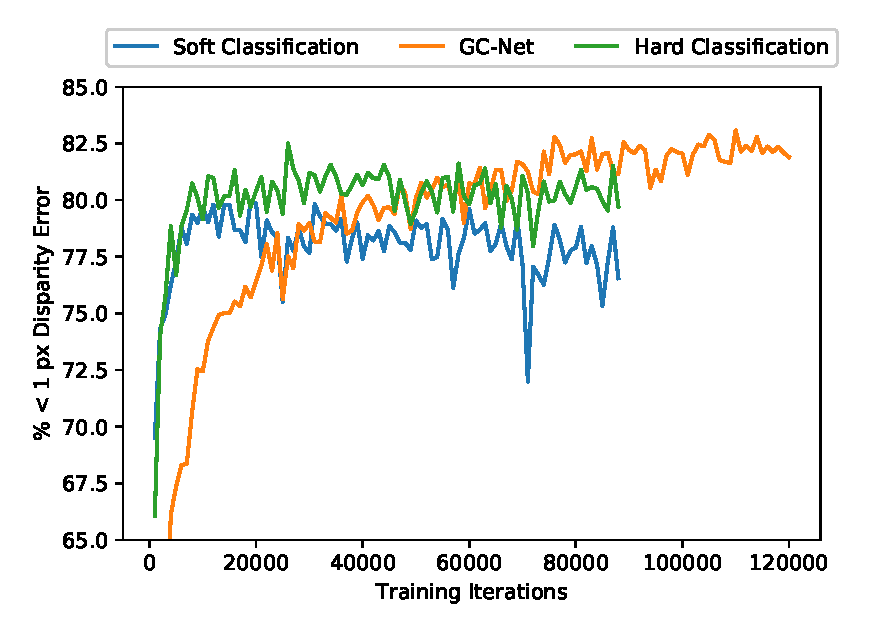
\includegraphics[width=0.66\linewidth]{training_plot.eps}
\caption[Validation error during training with the Scene Flow dataset.]{\textbf{Validation error} (percentage of disparities with error less than 1 px) during training with the Scene Flow dataset. Classification loss trains faster, however using a regression loss results in better performance.}
\label{fig:training_err}
\end{figure}

\fig{training_err} plots validation error during training for each of the networks compared in this section. We observe that the classification loss converges faster, however the regression loss performs best overall.

\subsection{KITTI Benchmark}
\label{sec:kitti_results}

\begin{table*}[t]
\centering
\begin{subtable}[t]{\linewidth}
\centering
\resizebox{\linewidth}{!}{
\begin{tabular}{l|cc|cc|cc|cc|c} \hline
& \multicolumn{2}{c|}{\textgreater 2 px} & \multicolumn{2}{c|}{\textgreater3 px} & \multicolumn{2}{c|}{\textgreater 5 px} & \multicolumn{2}{c|}{Mean Error} & Runtime \\
& Non-Occ & All & Non-Occ & All & Non-Occ & All & Non-Occ & All & (s) \\ \hline \hline
SPS-st \citep{yamaguchi2014efficient}  		& 4.98 & 6.28 & 3.39 & 4.41 & 2.33 & 3.00 & 0.9 px & 1.0 px & 2 \\
Deep Embed \citep{chen2015deep} 			& 5.05 & 6.47 & 3.10 & 4.24 & 1.92 & 2.68 & 0.9 px & 1.1 px & 3 \\
Content-CNN \citep{luo2016efficient}  		& 4.98 & 6.51 & 3.07 & 4.29 & 2.03 & 2.82 & 0.8 px & 1.0 px & \textbf{0.7} \\ 
MC-CNN \citep{zbontar2016stereo} 			& 3.90 & 5.45 & 2.43 & 3.63 & 1.64 & 2.39 & 0.7 px & 0.9 px & 67 \\
PBCP \citep{Seki2016BMVC} 					& 3.62 & 5.01 & 2.36 & 3.45 & 1.62 & 2.32 & 0.7 px & 0.9 px & 68 \\
Displets v2 \citep{guney2015displets} 		& 3.43 & 4.46 & 2.37 & 3.09 & 1.72 & 2.17 & 0.7 px & 0.8 px & 265 \\ \hline
GC-Net (this work)           				& \textbf{2.71} & \textbf{3.46} & \textbf{1.77} & \textbf{2.30} & \textbf{1.12} & \textbf{1.46} & \textbf{0.6 px} & \textbf{0.7 px} & 0.9 \\
\end{tabular}}
	\caption{\textbf{KITTI 2012 test set results} \citep{Geiger2012CVPR}. This benchmark contains 194 train and 195 test gray-scale image pairs.}
	\label{tbl:kitti2012}
\end{subtable}

\vspace{5 mm}

\begin{subtable}[t]{\linewidth}
\centering
\resizebox{\linewidth}{!}{
\begin{tabular}{l|ccc|ccc|c} \hline
                   & \multicolumn{3}{c|}{All Pixels} & \multicolumn{3}{c|}{Non-Occluded Pixels} & Runtime \\
                   & D1-bg   & D1-fg   & D1-all  & D1-bg   & D1-fg   & D1-all  & (s)     \\ \hline \hline
MBM \citep{einecke2015multi}			& 4.69 & 13.05 & 6.08 & 4.33 & 12.12 & 5.61 & 0.13 \\
ELAS \citep{geiger2010efficient} 	& 7.86 & 19.04 & 9.72 & 6.88 & 17.73 & 8.67 & 0.3 \\
Content-CNN \citep{luo2016efficient} & 3.73 & 8.58  & 4.54 & 3.32 & 7.44  & 4.00 & 1.0 \\
DispNetC \citep{MIFDB16} 			& 4.32 & \textbf{4.41}  & 4.34 & 4.11 & \textbf{3.72}  & 4.05 & \textbf{0.06}\\
MC-CNN \citep{zbontar2016stereo}     & 2.89 & 8.88  & 3.89 & 2.48 & 7.64  & 3.33 & 67  \\
PBCP \citep{Seki2016BMVC} 			& 2.58 & 8.74  & 3.61 & 2.27 & 7.71  & 3.17 & 68  \\
Displets v2 \citep{guney2015displets}& 3.00& 5.56  & 3.43 & 2.73 & 4.95  & 3.09 & 265 \\ \hline
GC-Net (this work)					& \textbf{2.21} & 6.16  & \textbf{2.87} & \textbf{2.02} & 5.58  & \textbf{2.61} & 0.9 \\      
\end{tabular}}
	\caption{\textbf{KITTI 2015 test set results} \citep{Menze2015CVPR}. This benchmark contains 200 training and 200 test color image pairs. The qualifier `bg' refers to background pixels which contain static elements, `fg' refers to dynamic object pixels, while `all' is all pixels (fg+bg). The results show the percentage of pixels which have greater than three pixels or 5\% disparity error from all 200 test images.}
	\label{tbl:kitti2015}
\end{subtable}
	\caption[Comparison to other stereo methods on the KITTI benchmark.]{Comparison to other stereo methods on the test set of \textbf{KITTI 2012 and 2015 benchmarks} \citep{Geiger2012CVPR,Menze2015CVPR}. Our method sets a new state-of-the-art on these two competitive benchmarks, out performing all other approaches.}
	\label{tbl:kitti_test}
\end{table*}

\begin{figure*}[p]
	\begin{center}
    		\begin{subfigure}[t]{\linewidth}
            \centering
			\includegraphics[width=0.31\linewidth]{results_kitti_2012/000000_10.png}
			\includegraphics[width=0.31\linewidth]{results_kitti_2012/000000_10_disp.png}
			\includegraphics[width=0.31\linewidth]{results_kitti_2012/000000_10_error.png}
            \vspace{1 mm}
			\includegraphics[width=0.31\linewidth]{results_kitti_2012/000005_10.png}
			\includegraphics[width=0.31\linewidth]{results_kitti_2012/000005_10_disp.png}
			\includegraphics[width=0.31\linewidth]{results_kitti_2012/000005_10_error.png}
            \vspace{1 mm}
			\includegraphics[width=0.31\linewidth]{results_kitti_2012/000016_10.png}
			\includegraphics[width=0.31\linewidth]{results_kitti_2012/000016_10_disp.png}
			\includegraphics[width=0.31\linewidth]{results_kitti_2012/000016_10_error.png}
	        \caption{KITTI 2012 test data qualitative results. From left: left stereo input image, disparity prediction, error map.}
            \vspace{2 mm}
		\end{subfigure}
    		\begin{subfigure}[t]{\linewidth}
            \centering
			\includegraphics[width=0.31\linewidth]{results_kitti_2015/000013_10.png}
			\includegraphics[width=0.31\linewidth]{results_kitti_2015/000013_10_disp.png}
			\includegraphics[width=0.31\linewidth]{results_kitti_2015/000013_10_error.png}
            \vspace{1 mm}
			\includegraphics[width=0.31\linewidth]{results_kitti_2015/000009_10.png}
			\includegraphics[width=0.31\linewidth]{results_kitti_2015/000009_10_disp.png}
			\includegraphics[width=0.31\linewidth]{results_kitti_2015/000009_10_error.png}
            \vspace{1 mm}
			\includegraphics[width=0.31\linewidth]{results_kitti_2015/000004_10.png}
			\includegraphics[width=0.31\linewidth]{results_kitti_2015/000004_10_disp.png}
			\includegraphics[width=0.31\linewidth]{results_kitti_2015/000004_10_error.png}
	        \caption{KITTI 2015 test data qualitative results. From left: left stereo input image, disparity prediction, error map.}
            \vspace{2 mm}
		\end{subfigure}
    		\begin{subfigure}[t]{\linewidth}
            \centering
			\includegraphics[width=0.31\linewidth]{results_scene_flow_test/1351_input.png}
			\includegraphics[width=0.31\linewidth]{results_scene_flow_test/1351_disp.png}
			\includegraphics[width=0.31\linewidth]{results_scene_flow_test/1351_gt.png}
            \vspace{1 mm}
			\includegraphics[width=0.31\linewidth]{results_scene_flow_test/2145_input.png}
			\includegraphics[width=0.31\linewidth]{results_scene_flow_test/2145_disp.png}
			\includegraphics[width=0.31\linewidth]{results_scene_flow_test/2145_gt.png}
            \vspace{1 mm}
			\includegraphics[width=0.31\linewidth]{results_scene_flow_test/2758_input.png}
			\includegraphics[width=0.31\linewidth]{results_scene_flow_test/2758_disp.png}
			\includegraphics[width=0.31\linewidth]{results_scene_flow_test/2758_gt.png}
	        \caption{Scene Flow test set qualitative results. From left: left stereo input image, disparity prediction, ground truth.}
		\end{subfigure}
	\end{center}
	\caption[Qualitative results.]{\textbf{Qualitative results.} By learning to incorporate wider context our method is often able to handle challenging scenarios, such as reflective, thin or texture-less surfaces. By explicitly learning geometry in a cost volume, our method produces sharp results and can also handle large occlusions.}
	\label{fig:results_qualitative}
\end{figure*}

In \tbl{kitti_test} we evaluate the performance of our model on the KITTI 2012 and 2015 stereo datasets \citep{Geiger2012CVPR,Menze2015CVPR}. These consist of challenging and varied road scene imagery collected from a test vehicle. Ground truth depth maps for training and evaluation are obtained from LIDAR data. KITTI is a prominent dataset for benchmarking stereo algorithms. The downside is that it only contains $200$ training images, which handicaps learning algorithms. for this reason, we pre-train our model on the large synthetic dataset, Scene Flow \citep{MIFDB16}. This helps to prevent our model from over-fitting the very small KITTI training dataset. We hold out 40 image pairs as our validation set.

\tbl{kitti2012} and \ref{tbl:kitti2015} compare our method, GC-Net (\underline{G}eometry and \underline{C}ontext \underline{Net}work), to other approaches on the KITTI 2012 and 2015 datasets, respectively\footnote{Full leaderboard:~\url{www.cvlibs.net/datasets/kitti/}}. Our method achieves state of the art results for both KITTI benchmarks, by a notable margin. We improve on state-of-the-art by 9\% and 22\% for KITTI 2015 and 2012 respectively. Our method is also notably faster than most competing approaches which often require expensive post-processing. In \fig{results_qualitative} we show qualitative results of our method on KITTI 2012, KITTI 2015 and Scene Flow.

Our approach outperforms previous deep learning patch based methods \citep{zbontar2015computing,luo2016efficient} which produce noisy unary potentials and are unable to predict with sub-pixel accuracy. For this reason, these algorithms do not use end-to-end learning and typically post-process the unary output with SGM regularization \citep{einecke2015multi} to produce the final disparity maps.

The closest method to our architecture is DispNetC \citep{MIFDB16}, which is an end-to-end regression network pre-trained on SceneFlow. However, our method outperforms this architecture by a notable margin for \textit{all} test pixels. DispNetC uses a 1-D correlation layer along the disparity line as an approximation to the stereo cost volume. In contrast, our architecture more explicitly leverages geometry by formulating a full cost volume by using 3-D convolutions and a soft argmin layer, resulting in an improvement in performance.

\subsection{Cross Dataset Generalization}
\label{sec:generalize}

In \tbl{generalize} we investigate our model's ability to generalize across unseen datasets. We observe that our model is able to perform amicably on KITTI test data, even when only trained on Scene Flow -- a dissimilar synthetic dataset.

\begin{table}[h]
\centering
\begin{tabular}{l|l|c|c}
Train data & Test data & \textgreater3 px & Mean Error \\ \hline \hline
%KITTI 2015 Train & KITTI 2015 Val & & \\
Scene Flow & KITTI 2015 Val & 18.6 & 2.23 \\
KITTI 2015 Train & KITTI 2015 Val & 1.50 & 0.59 \\
\end{tabular}
	\caption[Cross dataset performance.]{Cross dataset performance. These results show that our method is able to generalize reasonably well across unseen datasets.}
	\label{tbl:generalize}
\end{table}

\begin{figure}[p]
\clearpage
	\begin{center}
    		\begin{subfigure}[t]{\linewidth}
            \centering
            \includegraphics[width=0.32\linewidth,trim={0 0 0 1cm},clip]{saliency/000005_10_png_input.png}
            \includegraphics[width=0.32\linewidth,trim={0 0 0 1cm},clip]{saliency/000016_10_png_input.png}
            \includegraphics[width=0.32\linewidth,trim={0 0 0 1cm},clip]{saliency/000074_10_png_input.png}
	        \caption{Left stereo input image}
		\end{subfigure}
    		\begin{subfigure}[t]{\linewidth}
            \centering
            \includegraphics[width=0.32\linewidth,trim={0 0 0 1cm},clip]{saliency/000005_10_png_disparity.png}
            \includegraphics[width=0.32\linewidth,trim={0 0 0 1cm},clip]{saliency/000016_10_png_disparity.png}
            \includegraphics[width=0.32\linewidth,trim={0 0 0 1cm},clip]{saliency/000074_10_png_disparity.png}
	        \caption{Predicted disparity map}
		\end{subfigure}
    		\begin{subfigure}[t]{\linewidth}
            \centering
            \includegraphics[width=0.32\linewidth,trim={0 0 0 1cm},clip]{saliency/000005_10_png_saliency.png}
            \includegraphics[width=0.32\linewidth,trim={0 0 0 1cm},clip]{saliency/000016_10_png_saliency.png}
            \includegraphics[width=0.32\linewidth,trim={0 0 0 1cm},clip]{saliency/000074_10_png_saliency.png}
	        \caption{Saliency map (red = stronger saliency)}
		\end{subfigure}
    		\begin{subfigure}[t]{\linewidth}
            \centering
            \includegraphics[width=0.32\linewidth,trim={0 0 0 1cm},clip]{saliency/000005_10_png_raw_frame_attenuated2.png}
            \includegraphics[width=0.32\linewidth,trim={0 0 0 1cm},clip]{saliency/000016_10_png_raw_frame_attenuated2.png}
            \includegraphics[width=0.32\linewidth,trim={0 0 0 1cm},clip]{saliency/000074_10_png_raw_frame_attenuated2.png}
	        \caption{What the network sees (input attenuated by saliency)}
		\end{subfigure}
	\end{center}
	\caption[Saliency map visualization.]{\textbf{Saliency map visualization} which shows the model's effective receptive field for a selected output pixel (indicated by the white cross). This shows that our architecture is able to learn to regress stereo disparity with a large field of view and significant contextual knowledge of the scene, beyond the local geometry and appearance. For example, in the example on the right we observe that the model considers contextual information from the vehicle and surrounding road surface to estimate disparity.}
	\label{fig:saliency_stereo}
\clearpage
\end{figure}

\subsection{Model Saliency}
\label{sec:saliency}

In this section we present evidence which shows our model can reason about local geometry using wider contextual information. In \fig{saliency_stereo} we show some examples of the model's saliency with respect to a predicted pixel's disparity. Saliency maps \citep{simonyan2013deep} shows the sensitivity of the output with respect to each input pixel. We use the method from \citep{zeiler2014visualizing} which plots the predicted disparity as a function of systematically occluding the input images. We offset the occlusion in each stereo image by the point's disparity.

These results show that the disparity prediction for a given point is dependent on a wide contextual field of view. For example, the disparity on the front of the car depends on the input pixels of the car and the road surface below. This demonstrates that our model is able to reason about wider context, rather than simply $9\times9$ local patches like previous deep learning patch-similarity stereo methods \citep{zbontar2016stereo,luo2016efficient}.

Next, we explore modelling uncertainty in stereo vision and show how to learn to regress depth with unsupervised learning.




\section{Uncertainty in Stereo Vision}

In this section, we present a method to model uncertainty in stereo vision using \textit{probabilistic deep learning}, which provides a framework for understanding uncertainty with deep learning models (\cref{scene_understanding}). In \sct{unc_model} we show how to form an architecture which learns to regress stereo disparities and \textit{heteroscedastic} (data dependent) uncertainty \citep{der2009aleatory} from a rectified stereo pair of images. Our method does not require labels for uncertainty, rather it is learned implicitly from the data. Unlike other probabilistic deep learning approaches \citep{gal2016thesis}, our method does not depend on drop-out sampling and is real-time.

We first review related work in stereo vision which considers uncertainty. Hand-engineered measures of uncertainty in matching costs are often used in stereo to improve disparity map prediction \citep{hu2012quantitative,egnal2004stereo}. Most uncertainty measures are designed to detect occlusions, surface discontinuities and texture-less regions. Hand designed approaches are common, for example using statistical approaches \citep{sabater2012meaningful}, measures of distinctiveness \citep{yoon2007stereo,manduchi1999distinctiveness} or entropy \citep{scharstein1998stereo}. Random forests have also be used to estimate matching cost confidence  \citep{Haeusler2013a,Park2015}. However, the use of uncertainty in stereo has predominantly been limited to estimating the confidence of matching costs to assist post-processing and regularization. In this section, we estimate the uncertainty of the final predicted disparity map.

\begin{figure*}[t]
\centering
\resizebox{0.9\linewidth}{!}{
  \begin{subfigure}[t]{0.5\linewidth}
      \includegraphics[width=\linewidth]{uncertainty/000160_10_png_input.png}
      \caption{Left stereo image input.}
  \end{subfigure}
  \begin{subfigure}[t]{0.5\linewidth}
      \includegraphics[width=\linewidth]{uncertainty/000160_10_right.png}
      \caption{Right stereo image input.}
  \end{subfigure}}
\vspace{1 mm}
\resizebox{0.9\linewidth}{!}{
  \begin{subfigure}[t]{0.5\linewidth}
      \includegraphics[width=\linewidth]{uncertainty/000160_10_png_disparity.png}
      \caption{Disparity output.}
  \end{subfigure}
  \begin{subfigure}[t]{0.5\linewidth}
      \includegraphics[width=\linewidth]{uncertainty/000160_10_png_uncertainty.png}
      \caption{Heteroscedastic uncertainty output.}
  \end{subfigure}}
\caption[Probabilistic deep learning model for stereo vision.]{\textbf{End-to-end probabilistic deep learning model for stereo disparity regression.} We observe increased uncertainty on occlusion boundaries and difficult surfaces, such as the red car's reflective and transparent windows.}
\label{fig:loss}
\end{figure*}

\subsection{Modelling Uncertainty in Stereo Vision}
\label{sec:unc_model}

In this section we introduce probabilistic deep learning, and show how to model uncertainty in stereo vision. In \cref{scene_understanding}, we explained there are two main types of uncertainty that one can model in Bayesian modelling \citep{der2009aleatory}. \textit{Aleatoric} uncertainty captures noise inherent in the observations. This could be due to sensor noise or variables the sensor is unable to capture, resulting in uncertainty which cannot be reduced even if more data were to be collected.
On the other hand, \textit{epistemic} uncertainty accounts for uncertainty in the model parameters -- uncertainty which captures our ignorance about which model generated our collected data.
This uncertainty can be explained away given enough data, and is often referred to as \textit{model uncertainty}. Aleatoric uncertainty can further be categorized into \textit{homoscedastic} uncertainty, uncertainty which stays constant for different inputs, and \textit{heteroscedastic} uncertainty. Heteroscedastic uncertainty depends on the inputs to the model, with some inputs potentially having more noisy outputs than others. 

\cref{scene_understanding} makes the observation that heteroscedastic uncertainty is especially important for computer vision applications. This is because epistemic uncertainty is often explained away by the availability of large datasets or unsupervised learning (\sct{unsupervised}). However, heteroscedastic uncertainty, which is uncertainty which is inherent to the data, is important to understand. For stereo vision, one can imagine the types of appearances which should have large heteroscedastic uncertainty, such as reflective surfaces, transparent objects, texture-less areas and over exposed image regions.

Importantly, many applications of stereo vision require algorithms to run in real-time. One of the attractive properties of modelling heteroscedastic uncertainty is that we can formulate probabilistic deep learning models which run in real-time \citep{kendall2017uncertainties}. In contrast, epistemic uncertainty is often intractable without sampling \citep{gal2016thesis}, which drastically increases the computational requirements of the model.

\subsection{Learning Heteroscedastic Uncertainty with Deep Learning}
\label{sec:bayes_loss}

In this section, we describe how to modify the GC-Net model (\cref{section:model}) into a probabilistic deep learning architecture to estimate heteroscedastic uncertainty in addition to disparity.

Homoscedastic regression (introduced in \cref{scene_understanding}) assumes constant observation noise, $\sigma$, for all input data. Heteroscedastic regression, on the other hand, assumes that observation noise can vary with input data \citep{nix1994estimating,le2005heteroscedastic}. Heteroscedastic models can be useful for stereo vision because parts of the observation space might have higher noise levels than others, such as reflective or textureless regions. Heteroscedastic uncertainty can be learned as a function of the data \citep{kendall2017uncertainties}. Therefore, variational inference is \textit{not} performed over the weights, but instead we perform maximum a posteriori inference -- finding a single value for the model parameters. This approach \textit{does not} allow us to capture epistemic model uncertainty, but has the advantage of being real-time and does not require Monte Carlo sampling.

To train a heteroscedastic neural network, we need to infer the posterior distribution by learning a function, $f$, which maps a pair of stereo input images, $I_{L}$ and $I_{R}$, to a disparity estimate, $\hat{d}$, and a measure of heteroscedastic uncertainty given by variance, $\hat{\sigma}^2$. 
\begin{equation}
[\hat{d}, \hat{\sigma}^2] = f(I_{L}, I_{R})
\end{equation}

The GC-Net model is designed to output disparity estimates, $\hat{d}$, by forming a cost volume of H$\times$W$\times$D$\times$1 dimensions, representing a cost for each disparity and pixel location. To adapt the architecture to regress an uncertainty measurement, $\hat{\sigma}^2$, we modify the final 3-D convolutional layer to regress a cost volume of H$\times$W$\times$D$\times$2 dimensions. The final dimension's first value still represents the cost, with the second value representing uncertainty. To form the final output, the first values are put through a soft argmin layer across the disparity dimension (see \citep{kendall2017end} for a description) to form the disparity estimates, $\hat{d}$. We average the second values across the disparity dimension to form uncertainty estimates, $\hat{\sigma}^2$. Both these outputs are of size H$\times$W.

In the following section we explain the loss function we use to learn to estimate disparity and heteroscedastic uncertainty. We use the losses derived in \cref{sect:hetero}. We fix a Gaussian likelihood to model our heteroscedastic uncertainty. This induces a minimization objective given labelled output points, $d$:
\begin{equation}
\mathcal{L}_{heteroscedastic} = \frac{1}{2N} \sum_i ||d_i-\hat{d}_i||\hat{\sigma}^{-2}_i + \frac{1}{2}\log{\hat{\sigma}^2_i}
\label{eqn:bayes_loss}
\end{equation}
where $N$ is the number of output pixels $\hat{d}_i$ corresponding to input image $I$, indexed by $i$. $\hat{\sigma}^2$ is the probabilistic neural network output for the predicted variance.

This loss consists of two components; the residual regression and an uncertainty regularization term. We do not need `uncertainty labels' to learn uncertainty. Rather, we only need to supervise the learning to predict disparity. We learn the variance, $\hat{\sigma}^2$, implicitly from the loss function. The second regularization term prevents the network from predicting infinite uncertainty (and therefore zero loss) for all data points.

In practice, we train the network to predict the log variance, $\hat{s}_i := \log \hat{\sigma}_i^2$: 
\begin{equation}
\mathcal{L}_{heteroscedastic} = \frac{1}{2N} \sum_i ||d_i-\hat{d}_i|| \exp (-\hat{s}_i) + \frac{1}{2}\hat{s}_i.
\label{eqn:aleatoric_regression_loss2}
\end{equation}
This is because it is more stable than regressing the variance, $\hat{\sigma}^2$, as the loss avoids a potential division by zero. The exponential mapping also allows us to regress unconstrained scalar values, where $\exp(-\hat{s}_i)$ is resolved to the positive domain giving valid values for variance.

In \tbl{scene_flow2} and \tbl{kitti_val} we show that modelling heteroscedastic uncertainty improves performance on the SceneFlow and KITTI datasets (experimental details are described in \sct{experiments}). We observe that allowing the network to predict uncertainty allows it effectively to temper the residual loss by $\exp(-\hat{s}_i)$, which depends on the data. This acts similarly to an intelligent robust regression function. It allows the network to adapt the residual's weighting, and even allows the network to learn to attenuate the effect from erroneous labels. This makes the model more robust to noisy data -- inputs for which the model learned to predict high uncertainty for will have a smaller effect on the loss.

The model is discouraged from predicting high uncertainty for all points -- in effect ignoring the data -- through the $\log \hat{\sigma}^2$ term. Large uncertainty increases the contribution of this term, and in turn penalizes the model. The model is also discouraged from predicting very low uncertainty for points with high residual error, as low $\hat{\sigma}^2$ will exaggerate the contribution of the residual and will penalize the model.

\section{Unsupervised Learning}
\label{sec:unsupervised}

Stereo vision is a critical component for the success of many animal and robotic vision systems. However, there are significant challenges to develop robust stereo algorithms which can be trusted in the wild. 
Today, the best performing stereo methods are based on end-to-end deep learning \citep{zbontar2016stereo,luo2016efficient,kendall2017end,MIFDB16}. These methods are, however, very data-hungry, requiring large datasets to achieve top performance \citep{MIFDB16}. In the real world, getting access to large quantities of high quality labelled depth data is extremely challenging. For example, one of the most prominent stereo datasets, KITTI \citep{Geiger2012CVPR}, only contains a few hundred labelled training images. Getting labelled data is challenging because structured light sensors only work indoors and LIDAR sensors are expensive and produce sparse labels. Large synthetic datasets have been proposed \citep{MIFDB16} however these do not always transfer to real world applications.

In the previous section we formulated a model to learn stereo disparities, with uncertainties, from labelled training data. In this section we show how to formulate stereo regression as an unsupervised learning problem using deep learning. 

Recently, Garg et al. \citep{garg2016unsupervised} showed how to learn monocular depth without labelled depth data by using photometric reprojection error. Their method was able to train on $10,000's$ of unlabelled KITTI images, much more than the $200$ images with ground truth labels. This work has catalysed many of the recent advances in geometry with deep learning. For example, in monocular depth regression \citep{garg2016unsupervised,monodepth17}, optical flow \citep{jason2016back,ren2017unsupervised}, localisation \citep{kendall2017posenet} and ego-motion \citep{zhou2017unsupervised}. This demonstrates that photometric reprojection loss has emerged as the dominant technique for learning geometry with unsupervised learning.

However, unsupervised learning methods do not perform as well as supervised regression \citep{garg2016unsupervised,kendall2017uncertainties}.
This is because unsupervised learning suffers from the aperture problem -- where correspondence is ambiguous due to lack of context \citep{hartley2000}. For example in stereo vision, it is impossible to uniquely determine correspondences between featureless regions like blank walls or sky without considering the wider context \citep{Hirschmuller2007}. Methods which learn from photometric reprojection error typically enforce a smoothing prior which results in smooth prediction across these regions with no training signal \citep{garg2016unsupervised,monodepth17,zhou2017unsupervised}. However this also results in equally blurred regions where there is good structure and training signal in the data. For this reason, naively combining supervised depth regression and unsupervised learning with reprojection error typically worsens performance.

Unsupervised learning for \textit{monocular} depth prediction using deep learning was first demonstrated by Garg et al~\citep{garg2016unsupervised}. They showed how unlabelled stereo pairs can be used to train a monocular depth estimation model. In this work, we believe we are the first to demonstrate unsupervised deep learning for stereo vision. One of the reasons why this is now possible is because of new models which can be trained end-to-end to regress stereo disparity \citep{kendall2017end,MIFDB16}. Previous deep learning models learned to classify disparities with a probability vector \citep{zbontar2016stereo,luo2016efficient}. This representation classifies the output in discrete disparity steps making it is less suitable for unsupervised learning.

Unlike other unsupervised approaches to learning depth \citep{garg2016unsupervised}, we show that our probabilistic model does not need any smoothing terms in the loss. This is because the probabilistic regression loss is able to learn to attenuate noisy data points which previously would have required the smoothing regularization term during training. This results in a sharper depth prediction image which is able to capture thinner structures. Additionally, we explore the use of combining unsupervised and supervised learning as a semi-supervised loss when sparse data labels are available.
We demonstrate an improvement in disparity accuracy over non-probabilistic deep learning baselines. 

Using the end-to-end stereo regression model described in \cref{section:model}, we formulate an unsupervised regression loss. We can use the model's disparity estimate to align the left image, $I_L$, with the right stereo image, $I_R$. If the predicted disparity is equal to the true disparity then the corresponding pixel locations in the left and right stereo image should have the same intensity. This loss is known as the \textit{photometric reprojection error} \citep{hartley2000}.

More formally, we obtain this loss by resampling the right stereo image, $I_R$, with estimated disparities, $\hat{d}$. Using the sampling method proposed by spatial transformer networks \citep{jaderberg2015spatial}, this entire process is differentiable and able to be trained using back propagation. The photometric reprojection loss is given by:
\begin{equation}
\mathcal{L}_{photometric} = \frac{1}{N} \sum\limits_{u,v} \left\lVert I_L(u,v) - I_R(u-\hat{d}_{u,v},v) \right\rVert_1
\label{eqn:unsupervised_loss}
\end{equation}
where $I(u,v)$ represents the pixel intensity of image $I$ and $\hat{d}_{u,v}$ represents the estimated disparity, at pixel coordinate $(u,v)$.

However, this loss alone is noisy. The photometric reprojection error function is non-informative in homogeneous regions of the scene \citep{hartley2000} -- referred to as the aperture problem. For example, multiple disparities can generate equally good loss for repetitive or texture-less surfaces. For this reason, a prior is often applied to the loss function, typically a smoothing function, to overcome the aperture problem. Previous literature \citep{garg2016unsupervised} uses some form of the total variation (TV) loss \citep{rudin1992nonlinear}:
\begin{equation}
\mathcal{L}_{smooth} = \frac{1}{N} \sum\limits_{u,v} \left\lVert \nabla\hat{d}_{u,v} \right\rVert_1
\end{equation}
Combining this regularization loss with the photometric reprojection loss, yields the approach used by Garg et al. \citep{garg2016unsupervised} for unsupervised monocular depth regression:
\begin{equation}
\mathcal{L}_{unsupervised} = \mathcal{L}_{photometric} + \gamma \mathcal{L}_{smooth}
\label{eqn:smooth_loss}
\end{equation}
with weight $\lambda=0.01$. While this TV-regularized loss does indeed alleviate the aperture problem, and converge to a reasonable solution, it does over-smooth the output. In the monocular models, the predicted depth maps in the unsupervised case are over-smoothed and lose edge detail \citep{garg2016unsupervised}, compared to supervised regression models \citep{eigen2014depth}. \fig{qual_smooth} shows a similar result with stereo.

\subsection{Attenuating the Loss with Heteroscedastic \\Uncertainty}

In this section, we demonstrate that modelling heteroscedastic uncertainty can provide another solution to the aperture problem. Ideally, we would like to be able to learn to attenuate the photometric reprojection loss in areas of the image which are non-informative and suffer from the aperture problem. We would like to not regularize areas of the image which provide a good signal. This is in contrast to the TV-loss approach which smooths all areas equally.

Learning heteroscedastic uncertainty allows us to achieve this. We can interpret the loss in \eqn{bayes_loss} as learned attenuation \citep{kendall2017uncertainties}. Because the residuals are annealed by the learned variance, $\hat{\sigma}^2$, the model has the flexibility to recognize noisy or non-informative areas of the signal, and attenuate the training loss accordingly.

We can apply the heteroscedastic regression loss in \eqn{bayes_loss} to the photometric reprojection error loss in \eqn{aleatoric_regression_loss2} as follows:
\begin{multline}
\mathcal{L}_{heteroscedastic~unsupervised} = \frac{1}{2N} \sum_{u,v} \left\lVert I_L(u,v) - I_R(u-\hat{d}_{u,v},v) \right\rVert_1 \exp (-\hat{s}_{u,v}) + \frac{1}{2}\hat{s}_{u,v}
\label{eqn:aleatoric_unsupervised_loss}
\end{multline}

\tbl{scene_flow2} and \tbl{kitti_val} compare the performance of supervised learning against unsupervised learning with our heteroscedastic model on the Scene Flow and KITTI datasets (experimental details are described in \sct{experiments}). Unsupervised learning is more effective on synthetic data, because in real world data it is susceptible to camera noise. However, these results show that we can learn monocular depth unsupervised without a regularization or smoothing term. Empirically, we demonstrate an improved performance using the learned attenuation loss in \eqn{aleatoric_unsupervised_loss} over the regularized loss in \eqn{smooth_loss}. Qualitatively, we observe a sharper and more refined depth prediction.

\begin{table*}[t]
\centering
\resizebox{\linewidth}{!}{
\begin{tabular}{l|c|c|c|c|c|c|c|c}
Model Variant & \small Uncertainty & \small Unsupervised & \small Smooth Loss & Error & RMS & \small $>1px$ & \small $>3px$ & \small $>5px$ \\ \hline \hline
%
\multicolumn{9}{c}{\textit{Modelling heteroscedastic uncertainty improves performance:}} \\ \hline
GC-Net Baseline \citep{kendall2017end} & & & 							& 2.51 & 12.4 & 16.9 & 9.34 & 7.22\\
\textbf{+Heteroscedastic Uncertainty (this work)} & \checkmark & & 												& \textbf{2.16} & \textbf{10.5} & \textbf{15.0} & \textbf{8.76} & \textbf{6.85} \\
+Heteroscedastic (grey-scale input) & \checkmark & & 							& 2.84 & 14.9 & 16.7 & 9.82 & 7.62 \\ \hline
%
\multicolumn{9}{c}{\textit{Uncertainty can be used instead of a smoothing prior for unsupervised learning:}} \\ \hline
+Unsupervised & & \checkmark &  										& 9.99 & 26.0 & 50.3 & 25.8 & 23.2 \\
+Unsupervised+TV Loss & & \checkmark & \checkmark  						& 8.98 & \textbf{23.3} & 39.2 & 25.1 & 21.5 \\
+Unsupervised+Heteroscedastic & \checkmark & \checkmark 						& & 8.99 & 24.9 & \textbf{38.6} & 25.0 & 21.4 \\
+Unsupervised+Heteroscedastic+TV Loss & \checkmark & \checkmark & \checkmark 	& \textbf{8.97} & 24.5 & 40.4 & \textbf{24.1} & \textbf{20.8} \\ \hline
%
\multicolumn{9}{c}{\textit{Semi-supervised learning can achieve reasonable performance with few labels:}} \\ \hline
\small +Semi-supervised (50\% labels)+Heteroscedastic & \checkmark & \checkmark & & 2.99 & 15.1 & 19.8 & 12.1 & 9.86 \\
\small +Semi-supervised (25\% labels)+Heteroscedastic & \checkmark & \checkmark & & 3.97 & 15.6 & 21.5 & 13.2 & 10.8 \\
\small +Semi-supervised (10\% labels)+Heteroscedastic & \checkmark & \checkmark & & 4.77 & 16.2 & 26.3 & 15.8 & 12.7 \\
\small +Semi-supervised (5\% labels)+Heteroscedastic & \checkmark & \checkmark & & 5.44 & 16.7 & 27.2 & 17.3 & 14.4 \\
\end{tabular}}
\caption[Results on the Scene Flow dataset with uncertainty and unsupervised learning.]{Results on the Scene Flow dataset \citep{MIFDB16}. Our probabilistic model improves mean disparity error by approximately 15\% over the baseline by modelling heteroscedastic uncertainty. For unsupervised learning, we observe that our probabilistic loss is able to improve metrics which test fine-grained accuracy, showing that it can lead to accurate results. With semi-supervised learning, our model can still achieve accurate results, even with reduced availability of ground truth labels. By leveraging probabilistic modelling, we learn from both supervised and unsupervised losses without needing smoothing priors.}
\label{tbl:scene_flow2}
\end{table*}

\subsection{Semi-Supervised Learning}

We can also train models in a semi-supervised fashion when we have some data with labels, and some data without labels. For example, the KITTI dataset provides 200 labelled training images, with some hundred thousand unlabelled frames. These losses can be combined:
\begin{equation}
\mathcal{L}_{semi-supervised} = \mathcal{L}_{supervised} + \beta \mathcal{L}_{unsupervised}
\label{eqn:semi_supervised}
\end{equation}
with weighting factor, $\beta=0.1$. During training, we sample equally from the labelled and unlabelled datasets to form training mini-batches. 

\tbl{scene_flow2} compares models with no labels (unsupervised), various fractions of the labels, through to all labels (supervised). We observe an increase in performance as the amount of labels increases. \tbl{kitti_val} shows that the effect is less pronounced on KITTI with real-world data, however semi-supervised learning reduces the need for pretraining on the synthetic SceneFlow dataset.

\begin{table*}[t]
\centering
\resizebox{\linewidth}{!}{
\begin{tabular}{l|l|c|cc|ccccc} \hline
Probabilistic&& Pretrained & \multicolumn{2}{c|}{Training Data} & \multicolumn{5}{c}{Disparity Error} \\
Modelling & Loss & SceneFlow & Labelled & Unlabelled & MAE & RMS & $>1px$ & $>3px$ & $>5px$ \\ \hline \hline
\xmark		 		& Supervised		& \xmark	 & 160 	& 0 	& 0.572 & 1.57 & 10.6 & 1.81 & 1.00 \\
\xmark		 		& Supervised		& \cmark	 & 160 	& 0 	& \textbf{0.567} & 1.44 & 10.2 & 1.67 & 0.89 \\
\cmark& Supervised		& \xmark	 & 160 	& 0 	& 0.584 & 1.56 & 10.2 & 1.73 & 0.89 \\
\cmark& Supervised		& \cmark	 & 160 	& 0 	& 0.579 & 1.56 & \textbf{10.1} & \textbf{1.62} & \textbf{0.86} \\ \hline
		 		& Unsupervised		& \xmark	 & 0 	& 43,552 & 3.20 & 7.81 & 50.4 & 16.3 & 11.1 \\
\cmark& Unsupervised		& \xmark	 & 0 	& 43,552 & 2.55 & 6.50 & 45.1 & 15.0 & 9.44 \\
\cmark& Unsupervised		& \cmark	 & 0 	& 43,552 & 1.77 & 3.77 & 46.1 & 12.6 & 6.91 \\ \hline
\xmark		 		& Semi-supervised	& \xmark	 & 160 	& 43,552 & 0.647 & 1.62 & 12.0 & 1.99 & 0.99 \\
\cmark& Semi-supervised	& \xmark	 & 160 	& 43,552 & 0.590 & 1.59 & 11.5 & 1.70 & 0.94 \\
\cmark& Semi-supervised	& \cmark	 & 160 	& 43,552 & 0.572 & \textbf{1.43} & 10.9 & 1.66 & 0.90 \\
\end{tabular}}
	\caption[Results on KITTI with probabilistic model.]{\textbf{KITTI 2015 validation set results} \citep{Geiger2012CVPR}. The KITTI 2015 stereo dataset dataset contains 200 labelled training images, of which we randomly hold out 40 as a validation set, and report these results here. We also use the KITTI odometry dataset, which contains 43,552 unlabelled stereo frames. Modelling uncertainty improves results. Naively combining supervised and unsupervised training worsens performance. However using semi-supervised learning with our probabilistic model achieves better results, even without pretraining on the SceneFlow dataset \citep{MIFDB16}.  }
	\label{tbl:kitti_val}
\end{table*}

\begin{figure*}[p]
	\begin{center}
    	\begin{subfigure}[t]{\linewidth}
          \resizebox{\linewidth}{!}{
            \centering
			\includegraphics[width=0.25\linewidth]{uncertainty/scene_flow_unsupervised/136_input.png}
			\includegraphics[width=0.25\linewidth]{uncertainty/scene_flow_unsupervised/28_input.png}
			\includegraphics[width=0.25\linewidth]{uncertainty/scene_flow_unsupervised/56_input.png}
			\includegraphics[width=0.25\linewidth]{uncertainty/scene_flow_unsupervised/83_input.png}}
	        \caption{Input left stereo image.}
		\end{subfigure}
    	\begin{subfigure}[t]{\linewidth}
          \resizebox{\linewidth}{!}{
            \centering
			\includegraphics[width=0.25\linewidth]{uncertainty/scene_flow_unsupervised/136_gt.png}
			\includegraphics[width=0.25\linewidth]{uncertainty/scene_flow_unsupervised/28_gt.png}
			\includegraphics[width=0.25\linewidth]{uncertainty/scene_flow_unsupervised/56_gt.png}
			\includegraphics[width=0.25\linewidth]{uncertainty/scene_flow_unsupervised/83_gt.png}}
	        \caption{Ground truth disparity labels.}
		\end{subfigure}
    	\begin{subfigure}[t]{\linewidth}
          \resizebox{\linewidth}{!}{
            \centering
			\includegraphics[width=0.25\linewidth]{uncertainty/scene_flow_unsupervised/136_disp.png}
			\includegraphics[width=0.25\linewidth]{uncertainty/scene_flow_unsupervised/28_disp.png}
			\includegraphics[width=0.25\linewidth]{uncertainty/scene_flow_unsupervised/56_disp.png}
			\includegraphics[width=0.25\linewidth]{uncertainty/scene_flow_unsupervised/83_disp.png}}
	        \caption{Unsupervised regression with probabilistic modelling (this work).}
            \label{fig:qual_smooth}
		\end{subfigure}
	\end{center}
	\caption[Qualitative results of our unsupervised probabilistic deep learning model.]{Qualitative results of our unsupervised probabilistic deep learning model on the Scene Flow dataset. We observe that our model can accurately learn the geometry of the scene, and learns accurate disparity estimates, without labelled training data.}
	\label{fig:results_qualitative_unsupervised}
    
	\begin{center}
    	\begin{subfigure}[t]{\linewidth}
          \resizebox{\linewidth}{!}{
            \centering
			\includegraphics[width=0.33\linewidth]{uncertainty/000005_10_png_input.png}
			\includegraphics[width=0.33\linewidth]{uncertainty/000164_10_png_input.png}
			\includegraphics[width=0.33\linewidth]{uncertainty/000167_10_png_input.png}}
	        \caption{Input left stereo image.}
		\end{subfigure}
    	\begin{subfigure}[t]{\linewidth}
          \resizebox{\linewidth}{!}{
            \centering
			\includegraphics[width=0.33\linewidth]{uncertainty/000005_10_png_disparity.png}
			\includegraphics[width=0.33\linewidth]{uncertainty/000164_10_png_disparity.png}
			\includegraphics[width=0.33\linewidth]{uncertainty/000167_10_png_disparity.png}}
	        \caption{Estimated disparity.}
		\end{subfigure}
    	\begin{subfigure}[t]{\linewidth}
          \resizebox{\linewidth}{!}{
            \centering
			\includegraphics[width=0.33\linewidth]{uncertainty/000005_10_png_uncertainty.png}
			\includegraphics[width=0.33\linewidth]{uncertainty/000164_10_png_uncertainty.png}
			\includegraphics[width=0.33\linewidth]{uncertainty/000167_10_png_uncertainty.png}}
	        \caption{Estimated heteroscedastic uncertainty.}
		\end{subfigure}
	\end{center}
	\caption[Qualitative results on the KITTI 2015 test set using supervised learning.]{Qualitative results on the KITTI 2015 test set using supervised learning. Qualitatively, the heteroscedastic uncertainty captures noise due to occlusion boundaries, texture-less surfaces and erroneous regions of the disparity map.}
	\label{fig:results_qualitative_kitti}
\end{figure*}

\section{Benchmarking Uncertainty}
\label{sec:experiments}

In this section we quantitatively analyse the effectiveness of the measure of heteroscedastic uncertainty. We show that it is well calibrated and correlates strongly with metric error.

Firstly, \fig{precision_recall} compares precision recall curves for supervised and unsupervised models on the Scene Flow dataset. These curves plot the disparity accuracy against varying percentiles of uncertainty measurements. This shows that the estimate for uncertainty accurately reflects the prediction error of the heteroscedastic neural network model, because both curves are strictly decreasing functions. Practically speaking, we observe a very strong correlation between metric error and uncertainty.

\begin{figure}[h]
\centering
\includegraphics[width=0.5\linewidth,trim={0 0 0 3em},clip]{uncertainty/regression_precision_recall}
\caption[Precision-recall plots.]{Precision-recall plots for supervised and unsupervised models on the Scene Flow dataset. These curves demonstrate our heteroscedastic uncertainty can effectively capture accuracy, as precision decreases with increasing uncertainty.}
\label{fig:precision_recall}
\end{figure}

Secondly, \fig{calibration} shows the calibration of our supervised and unsupervised models on the Scene Flow dataset. To form calibration plots for probabilistic regression models, we plot the frequency of residuals against probabilities given by the predicted heteroscedastic distribution. So, given $N$ predicted disparities, $\hat{d}_i$, predicted variance, $\hat{\sigma}^2_i$, and ground truth labels, $d_i$, we can compute the residuals, $r_i=|d_i-\hat{d}_i|$. We then calculate the frequency of these residuals which lie within probability, $p$, using the predicted distribution (in our case, with the Gaussian distribution) with variance $\hat{\sigma}^2_i$.
%, such that: $\textnormal{freq}(p) = \frac{1}{N} \sum_i (r_i < CDF_{Laplace}(p) * \sigma_i$), where $CDF$ is the cumulative distribution function. 
A perfectly calibrated model should behave such that $\textnormal{freq}(p)=p$ which reasons that for a given probability tolerance of $p$, $p$ predictions will be correct.

We observe that our models are well calibrated with mean square errors of 0.0060 and 0.0075 for supervised and unsupervised, respectively. The uncertainty for the supervised model is the raw, uncalibrated heteroscedastic uncertainty predicted by the model. For the unsupervised model, we need to calibrate it to estimate variance of the disparity prediction (measured in pixels), because the unsupervised heteroscedastic uncertainty estimates the variance of the photometric reprojection residuals (measured in pixel intensity). To achieve this, we apply a linear scaling factor which we tune empirically.

\begin{figure}[h]
\centering
\includegraphics[width=0.5\linewidth]{uncertainty/calibration_plots_regression}
\caption[Uncertainty calibration plots.]{Uncertainty calibration plots for supervised and unsupervised models on the Scene Flow dataset. This plot shows how well uncertainty is calibrated, where perfect calibration corresponds to the line $y=x$, shown in black. We observe our estimates of uncertainty are well calibrated with low mean squared error of 0.0060 and 0.0075 for supervised and unsupervised models, respectively.}
\label{fig:calibration}
\end{figure}


\section{Conclusions}

In this chapter, we investigated the problem of stereo vision and estimating disparity from a rectified pair of stereo images. We briefly summarise the main conclusions within the three main themes of this dissertation.

\textbf{End-to-end learning.}
We propose a novel end-to-end deep learning architecture for stereo vision. It is able to learn to regress disparity directly, without any additional post-processing or regularization. We demonstrate the efficacy of our method on the KITTI dataset, setting a new state-of-the-art benchmark.

\textbf{Geometry.}
We show how to efficiently learn context in the disparity cost volume using 3-D convolutions. We show how to formulate it as a regression model using a soft argmin layer. This allows us to learn disparity as a regression problem, rather than classification, improving performance and enabling sub-pixel accuracy. We demonstrate that our model learns to incorporate wider contextual information.

We show that we can use stereo geometry to learn depth with unsupervised learning. We formulate a loss using the photometric reprojection error. We show how to use uncertainty to combine supervised and unsupervised depth losses.

\textbf{Uncertainty.}
We have shown how to form a stereo architecture with probabilistic deep learning. In summary, our approach is:
\begin{itemize}
\item Safe. Our probabilistic neural network can reason about heteroscedastic uncertainty, which we quantitatively show is well-calibrated.
\item Accurate. Our approach improves over the performance of the baseline model.
\item Fast. We do not require sampling for probabilistic neural network inference and can estimate uncertainty while adding negligible extra compute.
\item Scalable. We show how to use unsupervised and semi-supervised learning to train our model with unlabelled stereo data, without requiring a smoothing or regularization loss term.
\end{itemize}